\documentclass[a4paper,12pt]{article}
\usepackage[MeX]{polski}
\usepackage[utf8]{inputenc}
\usepackage{graphicx}

\title{Sammy Sosa}
\author{Paweł Kumorowski}

\begin{document}
\maketitle

\begin{figure}[h]
	\centering
		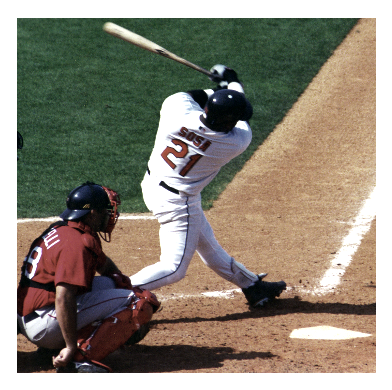
\includegraphics[width=0.6\textwidth]{sosa.eps}
		\caption{Sammy Sosa} \label{fig:sammy}

\end{figure}

\begin{abstract}
Samuel Peralta Sosa \ref{fig:sammy} (ur.~12~listopada~1968) --- dominikański baseballista, który występował na pozycji prawozapolowego przez 18~sezonów w Major~League~Baseball.
\end{abstract}

\tableofcontents

\section{Kariera zawodnicza}
W~lipcu~1985~roku podpisał kontrakt jako wolny agent z Texas~Rangers i~początkowo występował w klubach farmerskich tego zespołu, między innymi w~Oklahoma~City~89ers, reprezentujący poziom Triple-A. W~MLB zadebiutował 16~czerwca 1989~roku w~meczu przeciwko New York Yankees. W~Rangers wystąpił w~dwudziestu pięciu meczach i~jeszcze w~tym samym sezonie w~ramach wymiany przeszedł do~Chicago~White~Sox.

W~marcu 1992 podpisał kontrakt z~lokalnym rywalem White~Sox~Chicago~Cubs. W~sezonie 1993 został pierwszym zawodnikiem w~historii Cubs, który został członkiem Klubu 30–30, zdobywając 33` home runy i~36 skradzionych baz. Dwa lata później po raz pierwszy w~karierze wystąpił w~Meczu~Gwiazd i~ponownie osiągnął co~najmniej 30~home runów i~30~skradzionych baz. Został pierwszym baseballistą Cubs w~XX~wieku, który zwyciężał w~klasyfikacji pod względem zdobytych home runów i~skradzionych baz przez trzy kolejne sezony. W 1998~zdobył najwięcej w~National League runów (134), zaliczył najwięcej RBI (158) i~został wybrany najbardziej wartościowym zawodnikiem. W~latach 2000~i~2002~zwyciężał w~lidze w~klasyfikacji pod względem zdobytych home runów (odpowiednio 50~i~49), zaś w~sezonie 2001~zaliczył najwięcej RBI (158).

4 kwietnia 2003 w~meczu przeciwko Cincinnati~Reds zdobył 500.~home runa w karierze. W~lutym 2005~przeszedł do~Baltimore Orioles. W~tym samym roku, po~śledztwie przeprowadzonym w~firmie BALCo, przesłuchiwano baseballistów, w~tym Sosę, który przyznał, że~zażywał jedynie dozwolony środek kreatynę.

Rok później klub Washington~Nationals zaproponował mu występy w~klubach farmerskich tego zespołu jednak Sosa tę ofertę odrzucił, w~efekcie w~sezonie 2006~nie rozegrał żadnego spotkania. W~2007~rozegrał 114~meczów w~klubie, w~którym rozpoczynał swoją zawodową karierę, Texas~Rangers.

\section{Późniejszy okres}
W~2009~Sosa przyznał się, że~w~teście przeprowadzonym w~2003~roku na obecność środków niedozwolonych w~organizmie miał wynik pozytywny, jednak wówczas za pierwszy tego typu wynik w~zawodowym baseballu nie karano zawodników. Sosa powiedział, że~nigdy nie używał niedozwolonych środków dopingujących.

\section{Nagrody i wyróżnienia}
\begin{table}[h]
	\begin{tabular}{lc}
	\textbf{Nagroda/wyróżnienie}&\textbf{Lata}\\
	\hline
	MVP National League&1998\\
	7x All-Star&1995{, }1998{, }1999{, }2000{, }2001{, }2002{, }2004\\
	6x Silver Slugger Award&1995{, }1998{, }1999{, }2000{, }2001{, }2002\\
	Hank Aaron Award&1999\\
	Roberto Clemente Award&1998\\
	\hline
	\end{tabular}
\caption{nagrody i wyróżnienia}
\end{table}

\begin{thebibliography}{6}
\bibitem{label1}Sammy Sosa Transactions (ang.). baseball-reference.com. [dostęp 21 października 2012]
\bibitem{label2}1989 Oklahoma City 89ers (ang.). [dostęp 21 października 2012].
\bibitem{label3}Sammy Sosa Statistics (ang.). baseball-reference.com. [dostęp 21 października 2012].
\bibitem{label4}Rangers 3 Yankees 8 (ang.). baseball-reference.com. [dostęp 21 października 2012].
\bibitem{label5}Sammy Sosa's Biography (ang.). sammysosa.info. [dostęp 21 października 2012].
\bibitem{label6}Welcome to the 500 club, Sammy (ang.). cubs.com. [dostęp 21 października 2012].
\end{thebibliography}
\end{document}


